% Practice list C v4 --- Block 3, Question 6 (integrative, symbolic). Every result: practice-L5-L6-check-b3b.py

\questao{(15 points) Discursive. \emph{Integrative: growth $\times$ equilibrium interest rates $\times$ money demand $\times$
seigniorage $\times$ welfare.} An endowment economy produces $Y_t=Y_0(1+g)^t$, $Y_0>0$, $g\ge0$. A representative household
maximizes $\sum_{t\ge0}\beta^tc_t^{1-\sigma}/(1-\sigma)$ (logarithmic at $\sigma=1$), with $\sigma>0$ and $\beta\in(0,1)$, and
trades one-period real and nominal bonds, both in zero net supply. Real money demand is the reduced form $M_t/(P_tY_t)=\kappa e^{-ai_t}$,
$\kappa,a>0$, where $i_t$ is the nominal interest rate, and the Fisher relation holds exactly: $1+i_t=(1+r_t)(1+\pi_{t+1})$. The
government hands the new money to the household as a lump-sum transfer; with money growing at rate $\mu$ and new money valued
at today's prices, seigniorage is $S_t/Y_t=\mu\,M_t/(P_tY_t)$. Assume $\beta(1+g)^{1-\sigma}<1$ and study steady states
(constant $r$, $i$, $\pi$, $\mu$) with $i\ge0$. Brazil adopted inflation targeting in 1999 and has lived with high real interest
rates; the items ask what this economy says about both. All answers are symbolic.}

\textbf{a)} (3 points) Derive the Euler equation and find the equilibrium real interest rate. Show that
$\beta(1+g)^{1-\sigma}<1$ is the condition for household wealth to be finite and say what it implies for $r$ and $g$. Under a
money-growth rule $M_{t+1}=(1+\mu)M_t$, find steady-state inflation, the nominal rate and the admissible range of $\mu$.
\resolespaco
\begin{sol}
\passo{household problem}{With transfer $z_t$, real bonds $b_t$ and nominal bonds $B_t$ (in units of money), the budget is
$c_t+b_{t+1}+B_{t+1}/P_t=Y_t+z_t+(1+r_{t-1})b_t+(1+i_{t-1})B_t/P_t\equiv x_t$; money demand is a reduced form that does not enter
this choice. With $\mathcal L=\sum_t\beta^t\{u(c_t)+\lambda_t[x_t-c_t-b_{t+1}-B_{t+1}/P_t]\}$, where $\lambda_t$ is the marginal utility
of goods at $t$, the FOCs are $u'(c_t)=\lambda_t$, $\lambda_t=\beta(1+r_t)\lambda_{t+1}$ and $\lambda_t/P_t=\beta(1+i_t)\lambda_{t+1}/P_{t+1}$.
The first two give the Euler equation $c_t^{-\sigma}=\beta(1+r_t)c_{t+1}^{-\sigma}$; dividing the third by the second gives
$1+i_t=(1+r_t)(1+\pi_{t+1})$, the Fisher relation as no arbitrage between the two bonds.}
\passo{equilibrium}{Bonds are in zero net supply ($b_t=B_t=0$) and the transfer returns seigniorage, so goods clearing gives $c_t=Y_t$:
nobody can lend in the aggregate, and $r_t$ must make the household content to consume its endowment. Putting
$c_{t+1}/c_t=1+g$ into the Euler equation gives a constant rate,
\[1+r=\frac{(1+g)^{\sigma}}{\beta}.\]}
\passo{finite wealth}{Wealth is the present value of the endowment, $\sum_tY_t/(1+r)^t=Y_0\sum_t[(1+g)/(1+r)]^t$, finite iff
$(1+g)/(1+r)=\beta(1+g)^{1-\sigma}<1$, that is, iff $r>g$ (the same condition makes $\sum_t\beta^tu(Y_t)$ converge). Also $r>0$,
since $(1+g)^{\sigma}\ge1>\beta$.}
\passo{money and Fisher}{With $i$ constant, real balances $M_t/P_t=\kappa e^{-ai}Y_t$ grow at $g$, so $1+\mu=(1+\pi)(1+g)$; then
the Fisher relation gives
\[1+\pi=\frac{1+\mu}{1+g},\qquad 1+i=(1+r)(1+\pi)=\frac{(1+g)^{\sigma-1}(1+\mu)}{\beta}\equiv A\,(1+\mu),\]
where $A\equiv(1+r)/(1+g)=1/[\beta(1+g)^{1-\sigma}]>1$ by the assumption. Admissibility, $i\ge0$ (otherwise money dominates
bonds), is $1+\mu\ge1/A$, a bound below one: the money stock may shrink.}
\intuicao{With a representative agent, growth raises the real rate, not saving: everyone wants to borrow against a richer future,
and $r$ rises until nobody does. Money growth is split between output growth and inflation.}
\refbib{Kurlat (2020), ch.~6, \S6.2, eq.~(6.2.8); ch.~9, \S9.3, eq.~(9.3.14); ch.~11, \S11.1, eq.~(11.1.1), and \S11.2,
eq.~(11.2.3) with unit income elasticity; Romer (2012), ch.~2, \S2.5.}
\rubrica{
\item Budget, Lagrangian, FOCs and the Euler equation derived: 1 pt (Euler equation quoted: max.\ a third of this line).
\item $c_t=Y_t$ from clearing, $1+r=(1+g)^{\sigma}/\beta$, and finite wealth $\Leftrightarrow r>g$ proved: 1 pt.
\item $1+\pi$ from the money market, $1+i$ from the exact Fisher relation, admissible $\mu$: 1 pt. Using $r=1/\beta-1$ (no
growth) or log utility in place of the general case: max.\ half of the item.
}
\end{sol}

\textbf{b)} (3 points) Compare the money-growth rule with inflation targeting, in which the central bank sets money growth so
that $\pi=\pi^*$, with $\pi^*>0$. For each regime find $i$ and $\mu$, and prove for which $\sigma$ faster trend growth raises the
nominal rate. Decompose the response into the forces at work.
\resolespaco
\begin{sol}
\passo{money-growth rule}{From (a), $\ln(1+i)=(\sigma-1)\ln(1+g)+\ln(1+\mu)-\ln\beta$ with $\mu$ given, so
\[\frac{\partial i}{\partial g}=(1+i)\,\frac{\sigma-1}{1+g},\]
which has the sign of $\sigma-1$ because $1+i>0$: faster growth raises $i$ iff $\sigma>1$, leaves it unchanged at $\sigma=1$ and
lowers it iff $\sigma<1$. Inflation, $1+\pi=(1+\mu)/(1+g)$, falls with $g$ in every case.}
\passo{inflation targeting}{Now $\pi=\pi^*$ and $\mu$ is endogenous: the money-market step of (a) gives $1+\mu=(1+\pi^*)(1+g)$,
so $\partial\mu/\partial g=1+\pi^*>0$, and the Fisher relation gives
\[1+i=\frac{(1+g)^{\sigma}(1+\pi^*)}{\beta},\qquad\frac{\partial i}{\partial g}=(1+i)\,\frac{\sigma}{1+g}>0\quad\text{for every }\sigma>0.\]}
\passo{two forces}{Taking logs of $1+i=(1+r)(1+\pi)$,
\[\frac{d\ln(1+i)}{d\ln(1+g)}=\underbrace{\frac{d\ln(1+r)}{d\ln(1+g)}}_{=\,\sigma}
+\underbrace{\frac{d\ln(1+\pi)}{d\ln(1+g)}}_{=\,-1\text{ (rule)},\;0\text{ (target)}}.\]
Real-rate force ($\sigma$): faster income growth makes households want to borrow; since nobody can, $r$ rises, by more the lower
the intertemporal elasticity $1/\sigma$. Inflation force ($-1$): with $\mu$ fixed, real money demand grows with output and
absorbs part of the new money. Under the target the central bank supplies that money and the force vanishes, so the target's
elasticity exceeds the rule's by exactly one, whatever $\sigma$.}
\intuicao{Under a money rule growth is partly disinflationary, and at $\sigma=1$ the two forces cancel. Under a target only the
real-rate force is left: a central bank that targets inflation must raise $i$ when trend growth accelerates.}
\refbib{Kurlat (2020), ch.~11, \S11.2 and Exercise 11.5 (inflation targeting); Romer (2012), ch.~11, \S11.1.}
\rubrica{
\item Rule: $\partial i/\partial g$ in closed form and its sign $\Leftrightarrow\sigma\gtrless1$ proved: 1 pt (sign asserted
without the derivative: 0 for this line).
\item Target: $\mu$ endogenous, $i$, and $\partial i/\partial g>0$ for every $\sigma$: 1 pt.
\item Decomposition with both elasticities and their reading: 1 pt. Only one regime analysed: max.\ half of the item.
}
\end{sol}

\textbf{c)} (3 points) Under the money-growth rule, find the money growth rate $\mu^*$ that maximizes seigniorage, check the
second-order condition, prove that $\mu^*$ is the unique admissible maximizer, find the maximum revenue $s_{\max}$ in closed
form, and determine how trend growth moves the peak.
\resolespaco
\begin{sol}
\passo{revenue}{By (a), $i=A(1+\mu)-1$, so seigniorage is a tax rate $\mu$ times a base $\kappa e^{-ai}$ that shrinks with $\mu$:
\[s(\mu)\equiv\frac{S}{Y}=\kappa\,\mu\,e^{-a[A(1+\mu)-1]}.\]}
\passo{first-order condition}{$s'(\mu)=\kappa e^{-ai}(1-aA\mu)$ vanishes only at
\[\mu^*=\frac{1}{aA}=\frac{\beta(1+g)^{1-\sigma}}{a}>0,\]
where the elasticity of the base with respect to $\mu$, $-aA\mu$, equals $-1$.}
\passo{second order and uniqueness}{$s''(\mu)=\kappa aAe^{-ai}(aA\mu-2)$, so $s''(\mu^*)=-\kappa aAe^{-ai^*}<0$. Globally, $s'$ has
the sign of $1-aA\mu$, positive below $\mu^*$ and negative above, so $\mu^*$ is the unique maximizer. It is admissible:
$i^*=A(1+\mu^*)-1=(A-1)+1/a>0$ because $A>1$.}
\passo{maximum revenue}{Substituting $\mu^*$ and $i^*$,
\[s_{\max}=\kappa\mu^*e^{-ai^*}=\frac{\kappa}{aA}\,e^{-1-a(A-1)}
=\frac{\kappa\beta}{a(1+g)^{\sigma-1}}\exp\Big\{-1-a\Big[\frac{(1+g)^{\sigma-1}}{\beta}-1\Big]\Big\}.\]}
\passo{growth and the peak}{$\partial A/\partial g=(\sigma-1)A/(1+g)$. Hence $d\ln\mu^*/d\ln(1+g)=1-\sigma$ and
$\partial i^*/\partial g=(\sigma-1)A/(1+g)$; and since $\ln s_{\max}=\ln\kappa-\ln a-\ln A-1-a(A-1)$ has
$\partial\ln s_{\max}/\partial A=-(1/A+a)<0$,
\[\frac{\partial\ln s_{\max}}{\partial g}=-\frac{(\sigma-1)(1+aA)}{1+g}.\]
So $\mu^*$ and $s_{\max}$ fall with $g$ iff $\sigma>1$ (rise iff $\sigma<1$, constant at $\sigma=1$), while $i^*$ moves the
opposite way. Inflation at the peak, $1+\pi^L=(1+\mu^*)/(1+g)=\frac{1}{1+g}+\frac{\beta}{a(1+g)^{\sigma}}$, falls with $g$ for every
$\sigma>0$, both terms being decreasing.}
\intuicao{The base is real balances and the tax rate on holding them is $i$. With $\sigma>1$ growth raises $i$ at any $\mu$, so
the base is smaller and the peak comes earlier and lower; with $\sigma<1$ the inflation force dominates and the peak moves out.}
\refbib{Kurlat (2020), ch.~11, \S11.3, Exercises 11.3 (seignorage with growth) and 11.6 (Cagan money demand); Romer (2012),
ch.~11, \S11.9.}
\rubrica{
\item $s(\mu)$ with $i(\mu)$ from (a), FOC and $\mu^*$: 1 pt. Using $i=r+\mu$ as if $g=0$: max.\ half of the item.
\item $s''(\mu^*)<0$, global uniqueness and $i^*>0$: 1 pt (SOC asserted without $s''$: 0 for this line).
\item $s_{\max}$ in closed form and each effect of $g$ proved: 1 pt.
}
\end{sol}

\textbf{d)} (3 points) Measure the welfare cost of a steady state with nominal rate $i$, relative to the Friedman rule $i=0$, by
the Bailey area $W(i)$: the area under the inverse money-demand curve between the balances held at $i$ and at $i=0$. Find
$w(i)\equiv W(i)/Y$ in closed form, prove that it rises with $i$ and characterize it for small and large $i$. Find the inflation and
money growth rates that implement the Friedman rule. Under the target $\pi^*$, with nominal rate $i_T$, find the cost per unit of
seigniorage, average and marginal. Draw the demand curve and the cost at the target.
\resolespaco
\begin{sol}
\passo{inverse demand}{With $m\equiv M/(PY)$, $m(i)=\kappa e^{-ai}$ inverts to $i(m)=\frac1a\ln\frac{\kappa}{m}$ on $(0,\kappa]$:
the height is the marginal value of one more unit of real balances. Balances fall from $\kappa$ (at $i=0$) to $m(i)$.}
\passo{Bailey area}{Substituting $m=\kappa e^{-ax}$, $dm=-a\kappa e^{-ax}dx$, and integrating by parts,
\[w(i)=\int_{m(i)}^{\kappa}\frac1a\ln\frac{\kappa}{m}\,dm=\int_0^{i}a\kappa\,x\,e^{-ax}\,dx
=\kappa\Big[\frac{1-e^{-ai}}{a}-i\,e^{-ai}\Big],\]
which equals $\int_0^im(x)\,dx-i\,m(i)$: the surplus lost by holders net of the transfer $i\,m(i)$ to the issuer.}
\passo{shape}{$w'(i)=\kappa a\,i\,e^{-ai}>0$ for $i>0$ and $w'(0)=0$: the cost is second order at the Friedman rule.
$w''(i)=\kappa ae^{-ai}(1-ai)$: convex below $i=1/a$, concave above. Since $e^{-ax}\le1$ in the integrand,
$w(i)\le\kappa ai^2/2$ (the Harberger triangle), with ratio tending to one as $ai\to0$. Writing
$w=\frac{\kappa}{a}[1-(1+ai)e^{-ai}]$, the cost is bounded by $\kappa/a$ and tends to it as $i\to\infty$.}
\passo{Friedman rule}{$i=0$ requires $(1+r)(1+\pi_F)=1$:
\[1+\pi_F=\frac{\beta}{(1+g)^{\sigma}}<1,\qquad1+\mu_F=(1+\pi_F)(1+g)=\beta(1+g)^{1-\sigma}<1.\]
Deflation at the rate $r/(1+r)$ and a shrinking money stock although output grows; seigniorage $\kappa\mu_F<0$ must be raised by
other taxes.}
\passo{cost per unit of seigniorage}{At the target, $1+i_T=(1+g)^{\sigma}(1+\pi^*)/\beta$, $\mu_T=(1+\pi^*)(1+g)-1>0$ and
$s_T=\kappa\mu_Te^{-ai_T}$. Average cost:
\[\frac{w(i_T)}{s_T}=\frac{e^{ai_T}-1-ai_T}{a\,\mu_T}>0.\]
Marginal cost, raising $\pi^*$ ($di_T=(1+r)\,d\pi^*$, $d\mu_T=(1+g)\,d\pi^*$):
\[\frac{dw}{ds}=\frac{w'(i_T)(1+r)}{\kappa e^{-ai_T}[(1+g)-a\mu_T(1+r)]}=\frac{aA\,i_T}{1-aA\mu_T},\]
positive iff $\mu_T<\mu^*$ and unbounded as $\mu_T\uparrow\mu^*$.}
\begin{center}
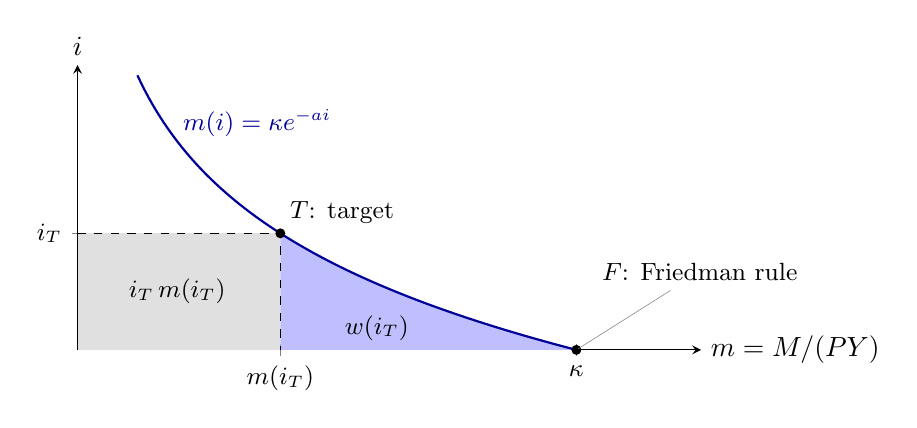
\begin{tikzpicture}
\begin{axis}[width=9.5cm,height=5.2cm,xmin=0,xmax=1.25,ymin=0,ymax=2.2,axis lines=left,clip=false,
  xtick={0.40657,1},xticklabels={$m(i_T)$,$\kappa$},ytick={0.9},yticklabels={$i_T$},
  xlabel={$m=M/(PY)$},ylabel={$i$},tick label style={font=\small},
  every axis x label/.style={at={(current axis.right of origin)},anchor=west},
  every axis y label/.style={at={(current axis.above origin)},anchor=south}]
\fill[black!12] (axis cs:0,0) rectangle (axis cs:0.40657,0.9);
\addplot[fill=blue!25,draw=none,domain=0.40657:1,samples=60] {ln(1/x)} \closedcycle;
\addplot[thick,blue!60!black,domain=0.12:1,samples=120] {ln(1/x)};
\draw[dashed] (axis cs:0,0.9) -- (axis cs:0.40657,0.9) -- (axis cs:0.40657,0);
\fill (axis cs:1,0) circle (1.8pt) node[inner sep=0pt,pin={[font=\small,pin distance=5ex]75:{$F$: Friedman rule}}] {};
\fill (axis cs:0.40657,0.9) circle (1.8pt) node[above right,font=\small] {$T$: target};
\node[font=\small] at (axis cs:0.6,0.17) {$w(i_T)$};
\node[font=\small] at (axis cs:0.2,0.45) {$i_T\,m(i_T)$};
\node[font=\small,blue!60!black] at (axis cs:0.36,1.75) {$m(i)=\kappa e^{-ai}$};
\end{axis}
\end{tikzpicture}
\end{center}
\intuicao{The cost depends on the nominal rate, not on inflation: with a high $r$, even a low $\pi^*$ means a sizeable $i_T$ and a
sizeable triangle, and the Friedman rule removes it only by deflating at about $r$.}
\refbib{Kurlat (2020), ch.~10, \S10.4; ch.~11, \S11.4 (the Friedman rule); Romer (2012), ch.~11, \S11.3 (``The Costs of
Inflation'').}
\rubrica{
\item $w(i)$ derived as the area under the inverse demand (or as $\int_0^im-i\,m(i)$), in closed form: 1 pt (formula quoted:
max.\ a third of this line).
\item $w'>0$, $w'(0)=0$, bounds, limits, $\pi_F$, $\mu_F$: 0.5 pt. Average and marginal cost per unit of seigniorage: 0.5 pt.
\item Graph (scored separately): axes $m$, $i$; a decreasing convex curve reaching $(\kappa,0)$; the area between $m(i_T)$ and
$\kappa$ shaded apart from the transfer rectangle; Friedman point marked: 1 pt (graph contradicting the algebra: 0).
}
\end{sol}

\textbf{e)} (3 points) \emph{Parameter analysis.} Sign the effects of $\sigma$, $g$, $\beta$, $a$ and $\kappa$ on $r$, on $i$ under
each regime, on $\mu^*$ and $s_{\max}$, and on the cost at the target, $w_T\equiv w(i_T)$, proving each sign or giving the
condition that decides it. Study $\sigma\to0$, $\sigma=1$, $g\to0$ and $a\to0$, and read the results for Brazil.
\resolespaco
\begin{sol}
\passo{log forms}{$\ln(1+r)=\sigma\ln(1+g)-\ln\beta$; $\ln(1+i)=(\sigma-1)\ln(1+g)+\ln(1+\mu)-\ln\beta$ (rule) and
$\sigma\ln(1+g)+\ln(1+\pi^*)-\ln\beta$ (target); $\ln\mu^*=\ln\beta+(1-\sigma)\ln(1+g)-\ln a$; $\ln s_{\max}=\ln\kappa-\ln a-\ln A
-1-a(A-1)$ with $\ln A=(\sigma-1)\ln(1+g)-\ln\beta$. So $\sigma$ enters through $\pm\ln(1+g)$, positive if $g>0$ and zero at
$g=0$; $g$ through $\sigma/(1+g)$ or $\pm(\sigma-1)/(1+g)$; $\beta$ through $\mp1/\beta$. For $s_{\max}$, chain through
$\partial\ln s_{\max}/\partial A=-(1/A+a)<0$; directly, $\partial\ln s_{\max}/\partial a=-1/a-(A-1)<0$. Neither $a$ nor $\kappa$
enters $r$ or $i$.}
\passo{cost at the target}{$w_T$ depends on $(\sigma,g,\beta)$ only through $i_T$, and $w'>0$, so it inherits the signs of $i$
under the target; it is proportional to $\kappa$. For $a$: $w_T=\kappa h(ai_T)/a$ with $h(x)=1-(1+x)e^{-x}$, so
$\partial w_T/\partial a=\kappa q(ai_T)/a^2$, where $q(x)\equiv xh'(x)-h(x)=(1+x+x^2)e^{-x}-1$. Since $q(0)=0$,
$q'(x)=x(1-x)e^{-x}$, $q(1)=3/e-1>0$, $q(2)=7/e^2-1<0$ and $q\to-1$, $q$ is positive on $(0,\hat x)$ and negative beyond its
unique positive root $\hat x\in(1,2)$: a more interest-elastic demand raises the cost iff $ai_T<\hat x$.}
\begin{center}
\begin{tabular}{lccccc}
\toprule
 & $\sigma$ & $g$ & $\beta$ & $a$ & $\kappa$\\
\midrule
$r$ & $+^{\dagger}$ & $+$ & $-$ & $0$ & $0$\\
$i$, money rule & $+^{\dagger}$ & $\operatorname{sgn}(\sigma-1)$ & $-$ & $0$ & $0$\\
$i$, target & $+^{\dagger}$ & $+$ & $-$ & $0$ & $0$\\
$\mu^*$ & $-^{\dagger}$ & $\operatorname{sgn}(1-\sigma)$ & $+$ & $-$ & $0$\\
$s_{\max}$ & $-^{\dagger}$ & $\operatorname{sgn}(1-\sigma)$ & $+$ & $-$ & $+$\\
$w_T$ & $+^{\dagger}$ & $+$ & $-$ & $+$ iff $ai_T<\hat x$ & $+$\\
\bottomrule
\end{tabular}

{\footnotesize $^{\dagger}$\,$0$ when $g=0$.}
\end{center}
\passo{limits and knife-edges}{$\sigma\to0$ (linear utility): $1+r\to1/\beta$ and no longer responds to growth; admissibility
becomes $\beta(1+g)<1$; under the rule $1+i\to(1+\mu)/[\beta(1+g)]$ falls with $g$ (only the inflation force is left) and
$\mu^*\to\beta(1+g)/a$ rises with $g$. $\sigma=1$ (log): $1+i=(1+\mu)/\beta$, $\mu^*=\beta/a$ and $s_{\max}$ do not depend on $g$,
because the two forces cancel; only under the target does $i$ rise with $g$. $g\to0$: $1+r\to1/\beta$, $\sigma$ drops out of
every result (its column becomes $0$), the regimes coincide when $\pi^*=\mu$, $1+\pi_F\to\beta$, $\mu^*\to\beta/a$ and
$s_{\max}\to\frac{\kappa\beta}{a}e^{-1-a(1/\beta-1)}$. $a\to0$: $w_T\le\kappa ai_T^2/2\to0$ and $\mu^*\to\infty$, so an
interest-inelastic demand has no distortion and no interior Laffer peak.}
\passo{reading for Brazil}{(i) High real rates: here $r$ is high only through impatience (low $\beta$) or fast growth priced with
a low elasticity (high $\sigma$ and $g$); with modest trend growth, a persistently high $r$ points to scarce saving (low $\beta$)
or to forces outside the model, such as risk premia. (ii) Inflation targeting: the policy rate tracks $r$ one for one
($d\ln(1+i)/d\ln(1+r)=1$), and meeting $\pi^*$ costs $w(i_T)$ with $1+i_T=(1+r)(1+\pi^*)$: a high real rate makes even a low
target costly, and the Friedman rule would demand deflation near $r$. (iii) Under the target seigniorage is a by-product,
$\mu_T=(1+\pi^*)(1+g)-1$; leaning on the inflation tax moves $\mu_T$ toward $\mu^*$, where the marginal cost explodes.}
\intuicao{Growth reaches $i$ through two channels of opposite sign and the regime decides whether the inflation channel
operates; welfare depends on $i$, hence on $r$, not on $\pi$ alone.}
\refbib{Kurlat (2020), ch.~9, \S9.3; ch.~11, \S\S11.2--11.4; Romer (2012), ch.~2, \S2.5; ch.~11, \S11.9.}
\rubrica{
\item Table complete and consistent with (a)--(d): 1 pt.
\item Each sign proved (log derivatives; $q(x)$ and $\hat x$ for $a$ on $w_T$): 1 pt (a sign without proof: 0 for that entry).
\item Limits $\sigma\to0$, $\sigma=1$, $g\to0$, $a\to0$ and the reading for Brazil: 1 pt. Signs without proofs or without the
reading: max.\ half of the item.
}
\end{sol}
